% ieeeaccess.cls reuses \year as a metadata setter. Preserve the TeX primitive
% so PGF/TikZ can initialize its deterministic machinery while loading.
\let\PSevenTeXYear\year
\documentclass{ieeeaccess}

% Shared packages and notation. Do not change IEEE Access class formatting here.
\usepackage{cite}
\usepackage{amsmath,amssymb,amsfonts}
\usepackage{graphicx}
\usepackage{textcomp}
\usepackage{bm}
\usepackage{booktabs}
\usepackage{array}
\usepackage{tabularx}
\usepackage{xcolor}
% The legacy IEEE Access class encodes its blue as a Pantone spot color that
% some current PDF renderers drop. Preserve the journal hue in device RGB so
% titles, section heads, and captions remain visible in archival renderers.
\definecolor{accessblue}{RGB}{0,114,178}
\let\PSevenIEEEAccessYear\year
\let\year\PSevenTeXYear
\usepackage{tikz}
\let\year\PSevenIEEEAccessYear
\usetikzlibrary{arrows.meta,positioning,fit,calc,shapes.geometric,backgrounds}
\usepackage[hidelinks]{hyperref}
\usepackage{etoolbox}

% ieeeaccess.cls adds an unnumbered REFERENCES entry to the PDF outline after
% creating the heading. Supply its hyperlink destination without altering the
% official class or its visual bibliography formatting.
\makeatletter
\patchcmd{\thebibliography}{\section*{\refname}}{\section*{\refname}\phantomsection}{}{}
\makeatother

% Replace the class template's published-volume placeholder with an honest
% circulation marker. The official class file itself remains unmodified.
\newcommand{\PSevenDraftFooter}{PREPRINT}
\makeatletter
\patchcmd{\ps@titlepage}{\footervolfont VOLUME\ \thevol, \theyear}{\footervolfont\PSevenDraftFooter}{}{}
\patchcmd{\ps@titlepage}{\footervolfont VOLUME\ \thevol, \theyear}{\footervolfont\PSevenDraftFooter}{}{}
\patchcmd{\ps@headings}{\footervolfont VOLUME\ \thevol, \theyear}{\footervolfont\PSevenDraftFooter}{}{}
\patchcmd{\ps@headings}{\footervolfont VOLUME\ \thevol, \theyear}{\footervolfont\PSevenDraftFooter}{}{}
\AtBeginDocument{\ps@headings}
\makeatother

\newtheorem{proposition}{Proposition}
\newtheorem{definition}{Definition}
\newtheorem{corollary}{Corollary}

\DeclareMathOperator*{\argmax}{arg\,max}
\DeclareMathOperator*{\argmin}{arg\,min}
\newcommand{\R}{\mathbb{R}}
\newcommand{\Pset}{\mathcal{P}}
\newcommand{\Hset}{\mathcal{H}}
\newcommand{\given}{\,|\,}

% Writing-assistance attribution, separate from scientific-source citations.
\newcommand{\AIDraftingCredit}{\footnote{Drafting/revision assistance:
OpenAI Codex~\cite{openaiCodex2026}.}}

\usepackage{pdfpages}
\usepackage{placeins}
\newcommand{\ObservedPMUCount}{8}
\newcommand{\HiddenBusCount}{31}
\newcommand{\NominalTestCount}{100}
\newcommand{\BZeroTVE}{0.3402\%}
\newcommand{\BOneTVE}{0.009904\%}
\newcommand{\BTwoTVE}{0.009634\%}
\newcommand{\BTwoRelativeImprovement}{2.7\%}
\newcommand{\BTwoMinusBOnePP}{-0.000270}
\newcommand{\BTwoMinusBOneCILowPP}{-0.000359}
\newcommand{\BTwoMinusBOneCIHighPP}{-0.000179}
\newcommand{\BTwoWinRate}{69.0\%}
\newcommand{\FunctionalSpearman}{0.5625}
\newcommand{\FunctionalSpearmanCILow}{0.271}
\newcommand{\FunctionalSpearmanCIHigh}{0.751}
\newcommand{\FunctionalPermutationP}{0.0012}
\newcommand{\FunctionalKendall}{0.376}
\newcommand{\MismatchMainCount}{980}
\newcommand{\MismatchRefinementCount}{175}
\newcommand{\NetworkMismatchRatio}{16.99}
\newcommand{\OperatingMismatchRatio}{8.32}
\newcommand{\OnlineClosurePercent}{0.4\%}
\newcommand{\UtwoNLL}{-16.184}
\newcommand{\UtwoCoverageRe}{93.9\%}
\newcommand{\UtwoCoverageIm}{94.2\%}
\newcommand{\OriginalInnovationACF}{0.602}
\newcommand{\MeasurementGMInnovationACF}{0.540}
\newcommand{\MismatchUzeroCoverage}{92.9\%}
\newcommand{\MismatchUtwoCoverage}{47.5\%}
\newcommand{\AdequacyHalfAUROC}{0.901}
\newcommand{\AdequacyHalfAUPRC}{0.779}
\newcommand{\AdequacyMaxAUROC}{0.928}
\newcommand{\AdequacyMaxAUPRC}{0.787}
\newcommand{\NetworkFrozenTVE}{0.250430\%}
\newcommand{\NetworkOracleTVE}{0.002547\%}
\newcommand{\NetworkOnlineTVE}{0.251132\%}
\newcommand{\OperatingFrozenTVE}{0.122641\%}
\newcommand{\OperatingOracleTVE}{0.001006\%}
\newcommand{\OperatingOnlineTVE}{0.122381\%}
\newcommand{\CoupledFrozenTVE}{0.023615\%}
\newcommand{\CoupledOracleTVE}{0.000396\%}
\newcommand{\CoupledOnlineTVE}{0.023615\%}
\newcommand{\EZeroHDevCount}{30}
\newcommand{\EZeroHTestCount}{60}
\newcommand{\EZeroHValidRate}{100.0\%}
\newcommand{\EZeroHClosureOverall}{98.1\%}
\newcommand{\EZeroHRuntimeMedian}{61.7}
\newcommand{\EZeroHRuntimePNinetyFive}{76.0}
\newcommand{\EZeroHRank}{25}
\newcommand{\EZeroHDimension}{43}
\newcommand{\EZeroHNullity}{18}
\newcommand{\EZeroHFunctionalResidual}{0.0419}
\newcommand{\EZeroHFrozenHalf}{0.19885\%}
\newcommand{\EZeroHFrozenOne}{0.38834\%}
\newcommand{\EZeroHFrozenMax}{0.57795\%}
\newcommand{\EZeroHCorrectedHalf}{0.00525\%}
\newcommand{\EZeroHCorrectedOne}{0.00749\%}
\newcommand{\EZeroHCorrectedMax}{0.00974\%}
\newcommand{\EZeroHClosureHalf}{97.4\%}
\newcommand{\EZeroHClosureOne}{98.1\%}
\newcommand{\EZeroHClosureMax}{98.3\%}
\newcommand{\EZeroHNEESHalf}{111.6}
\newcommand{\EZeroHNEESOne}{183.3}
\newcommand{\EZeroHNEESMax}{294.2}
\newcommand{\LegacyEventTrajectories}{690}
\newcommand{\LegacyEventDetectionFOne}{0.989}
\newcommand{\LegacyEventMacroFOne}{0.905}
\newcommand{\LegacyPhysicalTopOne}{0.592}
\newcommand{\LegacyPhysicalTopThree}{0.719}
\newcommand{\LegacyIntegrityTopOne}{0.974}
\newcommand{\LegacyFalseAlarmsPerMinute}{1.45}
\newcommand{\LegacyPhysicalGainPP}{9.6}
\newcommand{\LegacyPhysicalGainCILowPP}{6.9}
\newcommand{\LegacyPhysicalGainCIHighPP}{12.5}
\newcommand{\HeldSourceCorrect}{3}
\newcommand{\HeldSourceDecisions}{303}
\newcommand{\HeldSourceCases}{101}
\newcommand{\HeldSourceRate}{1.0\%}
\newcommand{\RawCandidateEventEpisodes}{2.7}
\newcommand{\RawCandidatePhysicalEpisodes}{0.3}
\newcommand{\LoadSourceCount}{16}
\newcommand{\LoadTangentMaxRelError}{0.235\%}
\newcommand{\LoadTangentMinCosine}{0.999995}
\newcommand{\LoadTangentMedianStressError}{1.56\%}
\newcommand{\LoadTangentMaxStressError}{4.55\%}
\newcommand{\LoadVOneEventCases}{2560}
\newcommand{\LoadVOneNoEventCases}{320}
\newcommand{\LoadVOneFPR}{0.625\%}
\newcommand{\LoadVOneTopOne}{100.0\%}
\newcommand{\LoadWeakEventCases}{9600}
\newcommand{\LoadWeakNoEventCases}{800}
\newcommand{\LoadFiniteEventCases}{8000}
\newcommand{\LoadTruncationSlope}{2.00}
\newcommand{\LoadTruncationCILow}{1.79}
\newcommand{\LoadTruncationCIHigh}{2.24}
\newcommand{\LoadWTwoNIS}{0.998}
\newcommand{\LoadWTwoACFOne}{-0.0026}
\newcommand{\LoadWTwoLjungP}{0.598}
\newcommand{\LoadLTwoDevCoverage}{95.0\%}
\newcommand{\LoadEVIRho}{-0.794}
\newcommand{\LoadProjectedFisherRho}{0.361}
\newcommand{\LoadWeakMinAUROC}{0.731}
\newcommand{\LoadWeakMinTopOne}{12.8\%}
\newcommand{\LoadFiniteCoverageMin}{92.9\%}
\newcommand{\LoadFiniteCoverageMax}{96.0\%}
\newcommand{\GlobalHypothesisCount}{137}
\newcommand{\GlobalPhysicalTrajectories}{3488}
\newcommand{\GlobalNoiseRecords}{10564}
\newcommand{\GlobalEventRecords}{10564}
\newcommand{\GlobalEventAUROC}{0.990}
\newcommand{\GlobalEventAUPRC}{0.9999}
\newcommand{\GlobalEventFNR}{7.3\%}
\newcommand{\GlobalEventFPRUpper}{3.6\%}
\newcommand{\GlobalWeakCardinality}{37.4\%}
\newcommand{\GlobalWeakTopOne}{24.4\%}
\newcommand{\GlobalWeakTopThree}{59.8\%}
\newcommand{\GlobalWeakStrongTopOne}{66.2\%}
\newcommand{\GlobalModerateTopOne}{98.8\%}
\newcommand{\GlobalFiniteTopOne}{100.0\%}
\newcommand{\GlobalInclusionAUROC}{0.950}
\newcommand{\GlobalInclusionECE}{0.029}
\newcommand{\WeakGlobalExactRho}{0.780}
\newcommand{\WeakSupportOnlyExactRho}{0.140}
\newcommand{\TOneTwentyGammaFour}{2844.44}
\newcommand{\TOneTwentyInfoRatio}{8.37}
\newcommand{\TOneTwentyCompleteMedianError}{0.0031}
\newcommand{\TOneTwentyCompleteMedianEta}{5.36e-04}
\newcommand{\TOneTwentyCompleteMaxEta}{0.088}
\newcommand{\TOneTwentyDMedianError}{0.2053}
\newcommand{\TOneTwentyDQMedianError}{0.4690}
\newcommand{\TOneTwentyHardPairSigma}{225.3}
\newcommand{\TOneTwentyHardPairCoherence}{0.999976}
\newcommand{\TOneTwentySevenTwelveCoherence}{-0.997947}
\newcommand{\TOneTwentyRuntime}{5.446}

\newcommand{\ContMixTimely}{53}
\newcommand{\ContMixTotal}{54}
\newcommand{\ContMixExtras}{4}
\newcommand{\ContMixOutTimely}{17}
\newcommand{\ContMixBusTimely}{2}
\newcommand{\ContNomTimely}{54}
\newcommand{\ContNomTotal}{54}
\newcommand{\ContNomExtras}{7}
\newcommand{\ContNomOutTimely}{18}
\newcommand{\ContNomBusTimely}{3}
\newcommand{\ContAdmissionTimely}{52}
\newcommand{\ContAdmissionTotal}{54}
\newcommand{\ContAdmissionExtras}{0}
\newcommand{\ContAdmissionOutTimely}{16}
\newcommand{\ContAdmissionBusTimely}{2}
\newcommand{\ContETTimely}{27}
\newcommand{\ContETTotal}{54}
\newcommand{\ContETExtras}{3}
\newcommand{\ContETOutTimely}{9}
\newcommand{\ContETBusTimely}{0}
\newcommand{\ContPriorTimely}{54}
\newcommand{\ContPriorExtras}{6}
\newcommand{\ChenMatchedCorrect}{299}
\newcommand{\ChenMatchedTotal}{300}
\newcommand{\ChenMatchedEarly}{1}
\newcommand{\ChenNormalExposure}{100,000}

\newcommand{\NarMixDetected}{54}
\newcommand{\NarMixJoint}{54}
\newcommand{\NarMixTimely}{53}
\newcommand{\NarMixEvents}{54}
\newcommand{\NarMixLoadTimely}{26}
\newcommand{\NarMixLoadTotal}{27}
\newcommand{\NarMixLineTimely}{27}
\newcommand{\NarMixLineTotal}{27}
\newcommand{\NarMixExtras}{4}
\newcommand{\NarNomDetected}{54}
\newcommand{\NarNomJoint}{54}
\newcommand{\NarNomTimely}{54}
\newcommand{\NarNomEvents}{54}
\newcommand{\NarNomLoadTimely}{27}
\newcommand{\NarNomLoadTotal}{27}
\newcommand{\NarNomLineTimely}{27}
\newcommand{\NarNomLineTotal}{27}
\newcommand{\NarNomExtras}{7}
\newcommand{\NarETDetected}{27}
\newcommand{\NarETJoint}{27}
\newcommand{\NarETTimely}{27}
\newcommand{\NarETEvents}{54}
\newcommand{\NarETLoadTimely}{0}
\newcommand{\NarETLoadTotal}{27}
\newcommand{\NarETLineTimely}{27}
\newcommand{\NarETLineTotal}{27}
\newcommand{\NarETExtras}{3}
\newcommand{\NarETSDetected}{27}
\newcommand{\NarETSJoint}{27}
\newcommand{\NarETSTimely}{27}
\newcommand{\NarETSEvents}{54}
\newcommand{\NarETSLoadTimely}{0}
\newcommand{\NarETSLoadTotal}{27}
\newcommand{\NarETSLineTimely}{27}
\newcommand{\NarETSLineTotal}{27}
\newcommand{\NarETSExtras}{3}
\newcommand{\NarWitnessDetected}{53}
\newcommand{\NarWitnessJoint}{53}
\newcommand{\NarWitnessTimely}{52}
\newcommand{\NarWitnessEvents}{54}
\newcommand{\NarWitnessLoadTimely}{25}
\newcommand{\NarWitnessLoadTotal}{27}
\newcommand{\NarWitnessLineTimely}{27}
\newcommand{\NarWitnessLineTotal}{27}
\newcommand{\NarWitnessExtras}{0}

\IfFileExists{generated/c01_macros.tex}{\input{generated/c01_macros}}{}

\begin{document}
\history{}
\doi{}

\title{Physics-Based Event Attribution From Sparse PMUs With Recovery Memory}
\author{\uppercase{Jorge Luis Mayorga Taborda}\authorrefmark{1}, \uppercase{Yessica Africano Rodriguez}\authorrefmark{1}, \uppercase{Masoud Barati}\authorrefmark{2}, \uppercase{Payman Dehghanian}\authorrefmark{3}, AND \uppercase{David Felipe Celeita Rodr\'iguez}\authorrefmark{4}}

\address[1]{Universidad de los Andes, Bogot\'a, Colombia}
\address[2]{Department of Electrical and Computer Engineering, University of Pittsburgh, Pittsburgh, PA, USA}
\address[3]{Department of Electrical and Computer Engineering, The George Washington University, Washington, DC, USA}
\address[4]{Faculty of Engineering, Universidad de La Sabana, Ch\'ia, Colombia}
\corresp{Corresponding author: Jorge Luis Mayorga Taborda (e-mail: jl.mayorga236@uniandes.edu.co).}

\markboth{Mayorga Taborda \headeretal, Sparse-PMU Attribution With Recovery Memory}{Mayorga Taborda \headeretal, Sparse-PMU Attribution With Recovery Memory}

\hypersetup{
  pdftitle={Recovery-Aware Physical Event Attribution From Sparse PMUs},
  pdfauthor={Jorge Luis Mayorga Taborda; Yessica Africano Rodriguez; Masoud Barati; Payman Dehghanian; David Felipe Celeita Rodriguez},
  pdfsubject={Causal physical event attribution, recovery, and source resolution from sparse PMUs},
  pdfkeywords={dynamic state estimation, functional observability, phasor measurement units, physics-informed inference, source localization}
}

\begin{abstract}
An electrical network can continue responding after an intervention is restored, while a new event begins before that response decays. With sparse PMUs, this creates ambiguity between a new source and the recovery of an earlier one. We formulate attribution through competing physical histories. The inference engine uses switched state-space predictors derived from the network differential-algebraic equations, together with voltage, terminal current, frequency and ROCOF from eight PMUs. It screens unknown onsets over a ten-second retrospective window, integrates load severity, and preserves separate active-event and originating-cause masses after restoration. A finite bank represents constant network-parameter uncertainty. \IfFileExists{generated/c01_macros.tex}{In the independent continuous evaluation, the five-model bank obtains \COneMixTimely{}/\COneMixTotal{} timely family/source decisions with \COneMixExtras{} unmatched alarms; nominal obtains \COneNomTimely{}/\COneNomTotal{} with \COneNomExtras{} extras.}{In completed development streams, the bank obtains \ContMixTimely{}/\ContMixTotal{} timely family/source decisions with \ContMixExtras{} unmatched alarms. Nominal gains one timely decision but produces more extras. The independent, prespecified evaluation remains in progress.} A separate known-onset load experiment illustrates why visible weak interventions can remain difficult to localize. The contribution is a specified recovery-aware attribution mechanism and an evaluation that separates detection, timely source decisions and restoration. The validated scope is a known load/line catalog; calibrated event probabilities, all-family diagnosis and real-time execution are not established.
\end{abstract}

\begin{keywords}
event detection, model uncertainty, phasor measurement units, physics-informed inference, sequential diagnosis, source localization.
\end{keywords}

\titlepgskip=-21pt
\maketitle

\section{Introduction}
\label{sec:introduction}

\PARstart{A}{n} unmeasured load changes. Several PMUs respond, a detector raises an alarm, and the network keeps oscillating after the load is restored. A second intervention then begins during that recovery. The operational question is no longer whether one signal exceeds a threshold: which physical intervention explains the reports observed so far, where did it originate, and when is that explanation distinguishable from the alternatives?

\begin{figure*}[t]\centering
\resizebox{\textwidth}{!}{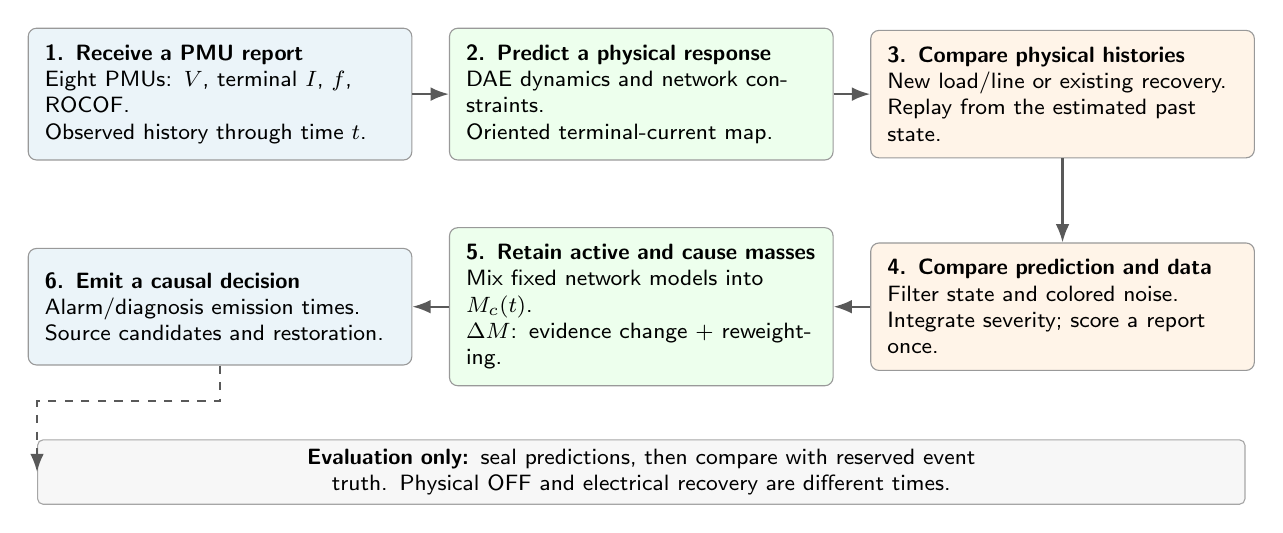
\begin{tikzpicture}[font=\sffamily\footnotesize\mdseries,>=Latex,
 box/.style={draw=black!40,rounded corners=3pt,align=left,text width=4.45cm,minimum height=1.48cm,inner sep=6pt},
 arr/.style={->,thick,draw=black!65}]
\node[box,fill=accessblue!8] (y) at (0,0) {\textbf{1. Receive a PMU report}\\Eight PMUs: $V$, terminal $I$, $f$, ROCOF.\\Observed history through time $t$.};
\node[box,fill=green!7] (physics) at (5.35,0) {\textbf{2. Predict a physical response}\\DAE dynamics and network constraints.\\Oriented terminal-current map.};
\node[box,fill=orange!9] (hyp) at (10.7,0) {\textbf{3. Compare physical histories}\\New load/line or existing recovery.\\Replay from the estimated past state.};
\node[box,fill=orange!9] (like) at (10.7,-2.7) {\textbf{4. Compare prediction and data}\\Filter state and colored noise.\\Integrate severity; score a report once.};
\node[box,fill=green!7] (mass) at (5.35,-2.7) {\textbf{5. Retain active and cause masses}\\Mix fixed network models into $M_c(t)$.\\$\Delta M$: evidence change + reweighting.};
\node[box,fill=accessblue!8] (out) at (0,-2.7) {\textbf{6. Emit a causal decision}\\Alarm/diagnosis emission times.\\Source candidates and restoration.};
\draw[arr] (y)--(physics);\draw[arr] (physics)--(hyp);\draw[arr] (hyp)--(like);\draw[arr] (like)--(mass);\draw[arr] (mass)--(out);
\node[draw=black!35,fill=black!3,rounded corners=2pt,align=center,text width=15.1cm,minimum height=.68cm] (eval) at (5.35,-4.8) {\textbf{Evaluation only:} seal predictions, then compare with reserved event truth. Physical OFF and electrical recovery are different times.};
\draw[arr,dashed] (out.south)--++(0,-.45)-|(eval.west);
\end{tikzpicture}
}
\caption{The complete scientific argument. Physics maps an intervention at an unmeasured source into predicted PMU trajectories; causal evidence chooses among those explanations. Event truth enters only evaluation. The figure describes the implemented restricted load/line component, not an already validated all-family joint estimator.}
\label{fig:joint-architecture}\end{figure*}

Sparse PMUs make the question difficult because a source need not have a sensor at its own bus. Its voltage, current and frequency effects propagate through the network \cite{phadke2008synchronized,zhao2019dse}. Uncertain operating context and network parameters can also change those effects. Moreover, physical OFF is not electrical recovery. A method that resets at restoration can treat the remaining response as another event or lose a real event that begins before the oscillation decays.

Strong existing methods solve parts of this problem. Dynamic state estimators combine power-system equations and PMU histories \cite{katanic2024recursive}; supervised classifiers learn sparse-PMU event/source labels \cite{pandey2020realtime,yildiz2024few}; physical outage detectors compare network hypotheses sequentially \cite{chen2016quickest,rovatsos2017outage}; and high-fidelity fault trajectories already support sparse-PMU diagnosis \cite{warner2023highfidelity}. The question here is how to retain an explanation through restoration and compare its recovery with a later intervention. A low state error does not prove source identity, and a score on represented assets does not prove source transfer.

Our approach uses the physical intervention as the object of inference.
DAE derivatives construct switched predictors for load and line candidates.
Starting from an estimated past state, those predictors describe what the
eight PMUs should report. Conditional likelihoods compare the predictions
with observations while accounting for severity and instrumental memory.
A finite network-model bank represents parameter uncertainty. Active and
originating-cause masses distinguish an ongoing intervention from the
response that remains after restoration.

The paper makes three scoped contributions:
\begin{enumerate}
\item \textbf{Recovery-aware physical attribution:} an executable causal load/line history bank starts from estimated past states, retains the originating cause after physical OFF, and compares recovery with new-intervention histories under fixed network hypotheses. We specify its evidence and publication rules.
\item \textbf{A qualified source-resolution analysis:} a separate archived load-support study exposes ambiguity and the different information used by joint and conditional source decisions. A prior-consistency audit distinguishes implementation effects from a claimed physical limit; this study is not counted as causal accuracy.
\item \textbf{A reproducible operational test:} the nominal/mixture comparison and a failed admission ablation expose the trade-off between timely source attribution and extra alarms. Separate state, batch and stream contracts retain their own denominators. R11 and nominal remain frozen co-references for confirmation.
\end{enumerate}

The central question is whether this recovery-aware construction preserves
timely source decisions without excessive extra alarms. The experiments
separate development from independent evaluation and keep detection,
eventual attribution and attribution before restoration as different
outcomes. Physical templates, onset scanning and Bayesian updates have
close precedents; the claimed contribution is their specified operational
construction for the declared load/line problem and its measured limits.



\section{Closest Methods and the Remaining Question}
\label{sec:narrative-related}

Dynamic state estimation supplies the state and uncertainty machinery used to predict a PMU history. Unknown-input and DAE estimators address incomplete models and exogenous inputs \cite{gillijns2007input,nugroho2022dae,katanic2024recursive}. Their task is not automatically an event-family/source decision. A recovered bus-voltage field can remain compatible with competing physical interventions.

Model-based source inference is the closest methodological precedent. Phasor angles support outage hypotheses \cite{tate2008outage}; uncertain pre-event conditions can be marginalized with outage identity \cite{zhao2014outages}; and sequential likelihoods detect line changes under stochastic operation \cite{chen2016quickest,rovatsos2017outage}. Transient dynamics and unknown onset are therefore established ingredients, not contributions of this paper.

Warner \emph{et al.} provide a particularly close precedent \cite{warner2023highfidelity}. Their simulated voltage/current fault trajectories are compared with a steady-state reference over a moving onset window; Algorithm~1 stops and returns candidate lines. Load changes are an adverse-event test rather than a load-source output. Their Sections~II and IV target short-circuit identification before clearing, whereas our restricted task follows load changes and line openings through restoration and later interventions. Sparse sensing, a physical trajectory library and retrospective onset scanning are shared ideas. We have not run their procedure on the present data and make no numerical superiority claim over it.

Sequential diagnosis also has a stronger statistical literature than a rolling-window label suggests. The Adaptive Matrix CuSum addresses misidentification caused by pre-change observations and establishes delay/error results under its specified observation laws \cite{warner2024matrix}. R11's pruned conditional histories, colored measurement state and plug-in startup estimates do not inherit those guarantees. A ten-second window or the array $M$ is not a replacement for that theory.

Learned PMU diagnosis provides a different comparator. Sparse classifiers and knowledge-driven representations identify represented events or assets \cite{pandey2020realtime,li2024knowledge,yildiz2024few}. The historical SGSMA baseline supplies two frozen ExtraTrees adaptations here. We distinguish interpolation at represented sources, transfer of that frozen adapter, and true held-source generalization. The present causal catalog is known; its results do not establish the last of those claims.

Observability and diagnosability explain why neither a physical nor learned method is guaranteed to localize every visible event. Functional observability concerns the requested state function \cite{fernando2010functional,montanari2022functional}; descriptor-model diagnosability and nuisance-profiled tests concern competing explanations \cite{eriksson2013diagnosability,scharf1994matched}. Placement-dependent source ambiguity is also established in PMU fault/event work \cite{jamei2020limits,conte2023fault,yildiz2025sparse}. Our state/source distinction applies these ideas; it is not their first discovery.

Multiple-model filtering already manages conditional state/mode hypotheses \cite{blom1988imm}; R11 is a pruned history bank, not a new IMM derivation. Stochastic swing/kernel models estimate latent states in Ensaf and Barati \cite{ensaf2023kernel}, and physics-derived prior covariances support sparse-state forecasting \cite{tartakovsky2023gp}. Joint DAE-aware generator/network parameter inference is studied separately \cite{albustami2026dae}. R11 uses a finite bank of constant network hypotheses rather than inferring the continuous parameter posterior. A Gaussian process or neural architecture would require separate validation.

\begin{table*}[t]\centering\small
\caption{Closest inference contracts and the difference tested here. This is a methodological comparison; only Chen and the frozen ExtraTrees adapters are executed comparators in C01. Absence from a paper's evaluated task is not a claim of algorithmic impossibility.}\label{tab:literature-capability}
\begin{tabularx}{\textwidth}{@{}lXXX@{}}\toprule
Route & Physical/statistical mechanism & Published target & Difference or role here\\\midrule
Chen / Rovatsos & Increment statistics, network models and sequential tests & Line outages; Rovatsos includes transient phases & Chen is executed on persistent-line first stops\\
Warner high-fidelity & Simulated V/I paths, moving onset window, distance evidence & Short-circuit line candidates & Nearest trajectory precedent; no common-data run here\\
Adaptive Matrix CuSum & Pairwise sequential diagnosis and error/delay analysis & One unknown change among distributional alternatives & No corresponding optimality guarantee is claimed here\\
DAE / stochastic-state estimation & Incomplete DAE observers or physical uncertainty models & States, unknown inputs or network parameters & Components/adjacent tasks, not episode attribution scores\\
Knowledge-driven learned diagnosis & Spatiotemporal representation with topology/type constraints & Multi-family disturbance location & Distinct from the physical likelihood; ExtraTrees is our executed learned reference\\
Physical history bank here & Estimated-past-state paths, active/cause masses, fixed R/X mixture & Successive known-catalog load/line interventions & Test whether recovery-aware attribution retains timely sources without excess alarms\\\bottomrule
\end{tabularx}\end{table*}

The remaining question is operational and falsifiable: can a state-conditioned bank distinguish a new intervention from a preceding intervention's recovery while retaining timely family/source decisions under fixed network uncertainty? Our contribution is the specified recovery-aware construction and its bounded evidence, not a claim to have invented model-based diagnosis. We use ``physics-informed'' because physical equations define candidate trajectories and likelihood inputs. Learned discrepancy and the unrestricted joint state/event/integrity estimator remain separate proposals.

\section{Problem and Measurement Model}
\label{sec:narrative-problem}

At report $k$, inference uses measurements through $t_k=k/30$ to decide
whether a physical intervention occurred. Detection concerns its presence;
classification selects a physical operator; localization selects a bus or
branch. These outputs can become reliable at different times. We record
the estimated physical onset $\widehat\tau$ separately from the alarm and
diagnosis emission times.

Figure~\ref{fig:reference-event-types} introduces the broader measurement
phenomena using the known RAW0001 reference record. Faults, line changes,
generation changes and load changes alter the physical network; missing or
corrupted reports alter observation integrity. The present causal test
addresses load changes and line openings with restoration. The other panels
provide context, not additional validated event classes.

\begin{figure*}[t]\centering
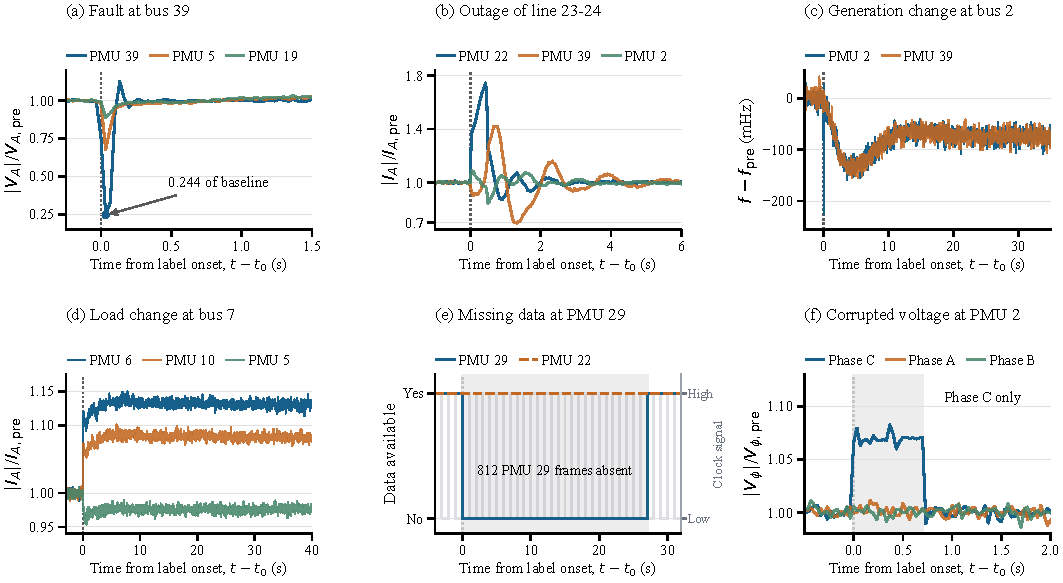
\includegraphics[width=.98\textwidth]{figures/generated/event_signatures.pdf}
\caption{Representative signatures from the archived RAW0001 reference simulation: fault, line outage, generation change, load change, missing PMU data and corrupted voltage. Alignment uses retrospective label onset for illustration; inference receives no such alignment. The gray clock in (e) is an illustrative reference, not another measured channel. Only load and line mechanisms enter the causal evaluation below. RAW0001 is known retrospective evidence, not independent field validation.}
\label{fig:reference-event-types}\end{figure*}

The network has 39 buses, but the prescribed PMU set is
\begin{equation}
 \mathcal P=\{2,5,6,10,19,22,29,39\}.
 \label{eq:narrative-pmus}
\end{equation}
Voltage is measured at each PMU bus. Current is measured at a specified branch terminal, which can differ from that bus. The causal implementation uses 47 coordinates: eight voltage magnitudes, eight voltage angles, eight current magnitudes, seven current angles, eight absolute frequencies and eight ROCOFs, at 30 reports/s. BUS39 current angle is excluded because its interpretation remains partially validated. The BUS5 current terminal retains the provisional historical 5--6 assignment. These are declared measurement assumptions, not identities inferred from classification accuracy.

The exported magnitudes are in V and A, angles in degrees, frequency in Hz
and ROCOF in Hz/s. Internal centered coordinates do not replace the
absolute frequency contract. These are reporting-rate phasor measurements;
waveform harmonics or THD are not measured by these channels.

% PROTECTED FIGURE: retain this single-column IEEE-39 diagram. See AGENTS.md.
\begin{figure}[t]\centering
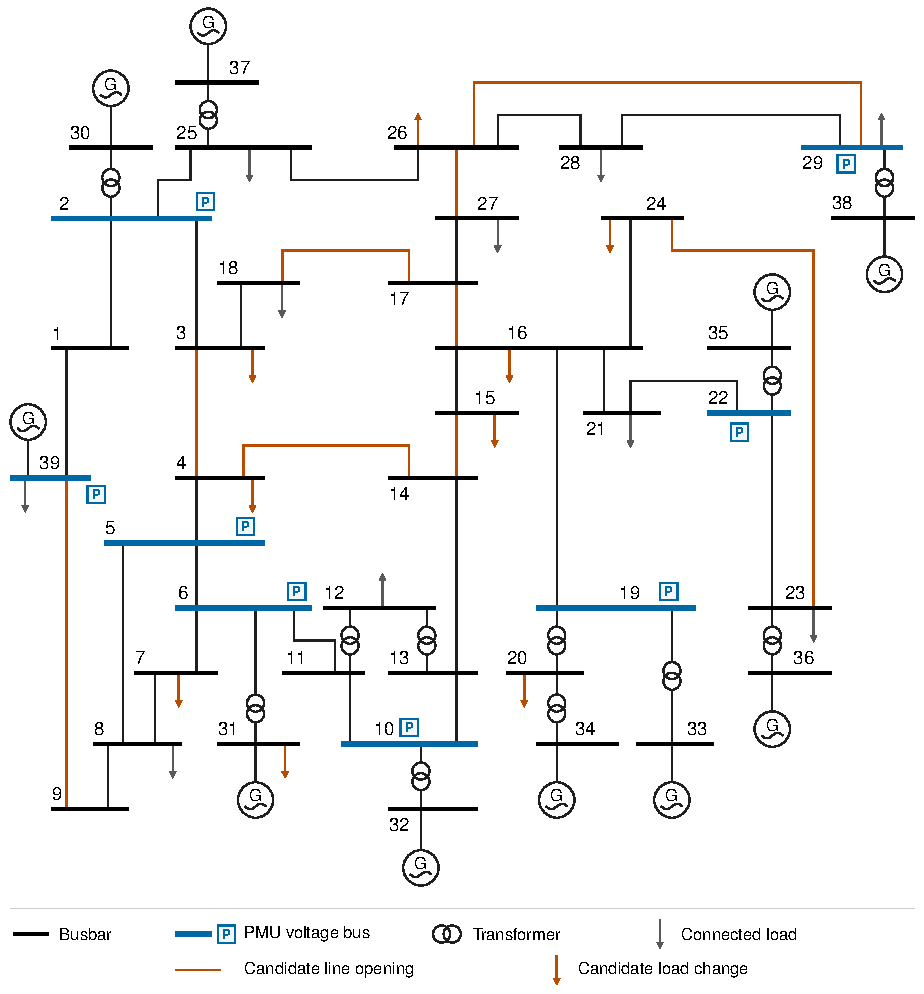
\includegraphics[width=\columnwidth]{figures/generated/narrative_topology.pdf}
\caption{IEEE 39-bus single-line diagram: 46 branches, 12 transformers and 10 generators. Blue bars and P marks locate the eight voltage PMUs. Orange branches and load arrows identify the nine line and nine load candidates; gray arrows denote other loads. Current terminals follow the separate measurement contract. All routes are orthogonal.}
\label{fig:narrative-topology}\end{figure}

The physical model is
\begin{align}
 \dot x&=f_q(x,z,u;\theta),&0&=g_q(x,z,u;\theta),\label{eq:narrative-dae}\\
 y_k&=\mathcal M_q(x_k,z_k;\theta_M)+b+\varepsilon_k.\label{eq:narrative-measurement}
\end{align}
Here $x$ contains machine and control dynamics, $z$ the algebraic network variables, $q$ the topology/intervention mode, and $\theta_M$ the measurement convention. The measurement map includes gains, phase references, orientation and the causal frequency/ROCOF estimator. A machine's rotor speed is not substituted for bus frequency.

An intervention history is $h=(e,c,\tau,a,\kappa)$: family, source, onset,
severity and restoration time, with $\kappa=\infty$ for a sustained event.
Its duration is $\kappa-\tau$ when restoration occurs. A load changes its
local P/Q setpoints; a line opening switches its branch primitive. For the
supported impulse-free switches,
\begin{equation}
 x(\tau^+)=x(\tau^-),\qquad g_{q^+}(x(\tau^-),z(\tau^+),u;\theta)=0.
 \label{eq:narrative-switch}
\end{equation}
The algebraic voltage/current response may jump even though dynamic states remain continuous. Physical restoration reverses the intervention operator. It does not return the machines to their pre-event state, so electrical recovery can continue after OFF.

\begin{table}[t]\centering\small
\caption{Scope of the executed causal component. The source is an intervention asset; it is not necessarily a measured PMU bus.}\label{tab:narrative-scope}
\begin{tabularx}{\columnwidth}{@{}lXX@{}}\toprule
Case & Physical operator & Executed claim\\\midrule
Normal & No intervention & Monitor after startup\\
Load & Local P/Q factor; optional restoration & Nine candidate buses\\
Line & Branch open; optional reclose & Nine candidate branches\\
Fault/generation & Different shunt/input/trip operators & Outside this causal test\\
Missing/bad data & Measurement-integrity mechanism & Outside C01\\
Unknown & Unresolved diagnosis & Not a new physical family\\\bottomrule
\end{tabularx}\end{table}

The generator stores event schedules and true states separately from the PMU stream. Inference receives the nominal network, permitted calibration and reports through the current time. It receives no source, switch time, true R/X realization or solver state. Initial operating context and noise scale are estimated from 300 startup reports; monitoring begins after the inherited 12-s warmup. The startup contract assumes no intervention in that prefix.

\section{Recovery-Aware Physical Attribution}
\label{sec:narrative-method}

Figure~\ref{fig:joint-architecture} describes the implemented computation.
The inference engine, archived as R11, uses a conditional history bank of
DAE-derived switched state-space predictors. The nonlinear simulator
generates observations; inference does not solve a new full nonlinear
simulation for every candidate at every report.

\subsection{Construct the Predictor From the Network}

Kirchhoff constraints and complex power connect sources to remote PMUs:
\begin{equation}
 I_{\rm bus}=Y_{\rm bus}V,\quad
 I_{{\rm term},r}=Y_{{\rm term},r}V,\quad S_i=V_i I_{{\rm bus},i}^{*}.
 \label{eq:narrative-electrical}
\end{equation}
Terminal rows retain orientation, line charging and transformer ratios.
A measured terminal current is not a nodal injection. A line opening
changes its branch primitive and terminal map; a load changes its admitted
P/Q input direction.

On a regular index-one DAE chart with a fixed angle reference,
\begin{align}
 \delta z&=-g_z^{-1}(g_x\delta x+g_u\delta u),\nonumber\\
 \delta\dot x&=A_q^{\rm red}\delta x+B_q^{\rm red}\delta u,\nonumber\\
 A_q^{\rm red}&=f_x-f_zg_z^{-1}g_x,\quad
 B_q^{\rm red}=f_u-f_zg_z^{-1}g_u.
 \label{eq:narrative-reduction}
\end{align}
Observation derivatives provide the corresponding reduced output. The
implementation discretizes these operators for the admitted switch modes.
Inertia, controls and load law remain those of the fixed plant.

After augmenting instrumental memory, a conditional predictor has the
local form
\begin{align}
 \xi_{k+1}&=A_{\ell,q}\xi_k+b_{\ell,q}+B_{\ell,q}a+w_k,\nonumber\\
 r_k&=C_{\ell,q}\xi_k+d_{\ell,q}+D_{\ell,q}a+v_k.
 \label{eq:implemented-predictor}
\end{align}
Here $r_k$ contains reference-corrected, scaled and instrument-whitened PMU coordinates, $\ell$ is a fixed
network hypothesis, and $\xi_k$ contains physical deviation states, phase
history and predicted measurement-filter memory. Observed colored-instrument
filters whiten measurements; their corresponding predictor memory is
deterministic. Additional latent AR states represent persistent discrepancy,
with preset quiet/load/line/recovery covariance and drift regimes. This
statistical discrepancy model is distinct from the plant equations.
$v_k$ denotes the remaining innovation. A load has scalar severity within
its specified P/Q direction. A line uses a switched operator rather than
a fictitious load-amplitude fit. States from different equilibria are not
interpreted as an absolute rotor-state mixture.

\subsection{Estimate Context From the Startup Prefix}

Each network hypothesis uses the same 300 startup reports to estimate
operating factors, reference phase and noise scale. Voltage/current
coordinates receive a constant discrepancy correction,
\begin{equation}
 \widehat b_\ell=\overline y_{0:299}-y_\ell^{\rm ref},
 \qquad b_{\ell,k}=\widehat b_\ell\quad(k\ge300).
 \label{eq:continuous-intercept}
\end{equation}
Angular differences respect wrapping and the common reference. Frequency
and ROCOF use empirical prefix centers. The correction remains fixed so it
cannot track a later load step and subtract its signature. This estimates
an observation discrepancy, not the true impedances. Prefix estimates
enter by substitution rather than through a full joint parameter posterior.

\subsection{Compare Unknown-Onset Histories}

At time $t_k$, the proposal screen considers onsets in
$[t_k-10\,\mathrm{s},t_k]$. Each history specifies family, asset, onset,
restoration mode and severity. It starts from the stored conditional state
before its proposed onset. That state already contains any ongoing
recovery; an alarm does not reset the predictor to equilibrium.

For a retained load history, conditional Gaussian filtering yields a
residual $e$, severity response $s$ and covariance $S$. Unknown severity
has a truncated-Gaussian distribution inherited from previous reports:
\begin{equation}
 L_{h,k}=\int_l^u \mathcal N(e;sa,S)
             \operatorname{TN}_{[l,u]}(a;\mu,v)\,da.
 \label{eq:narrative-evidence}
\end{equation}
With $\Phi$ denoting the standard normal CDF, define
\begin{align}
 v'&=(v^{-1}+s^\top S^{-1}s)^{-1},\nonumber\\
 \mu'&=v'(\mu/v+s^\top S^{-1}e),\nonumber\\
 Z(\mu,v)&=\Phi((u-\mu)/\sqrt v)-\Phi((l-\mu)/\sqrt v).
\end{align}
The implemented local integral follows by completing the square:
\begin{align}
 \log L_{h,k}&=\log\mathcal N(e;0,S)+\tfrac12\log(v'/v)\nonumber\\
 &\quad+\tfrac12(\mu'^2/v'-\mu^2/v)
       +\log\frac{Z(\mu',v')}{Z(\mu,v)}.
 \label{eq:amplitude-evidence-main}
\end{align}
These standard identities are exact for the stated local conditional
model. Adaptive proposals, pruning and covariance approximations make the
complete bank approximate.

The rolling screen proposes histories; it is not another independent
observation. Replaying a suffix replaces its original no-new-event suffix
likelihood. The sequential update therefore counts each report once,
rather than repeatedly accumulating overlapping ten-second windows.

\begin{figure*}[t]\centering
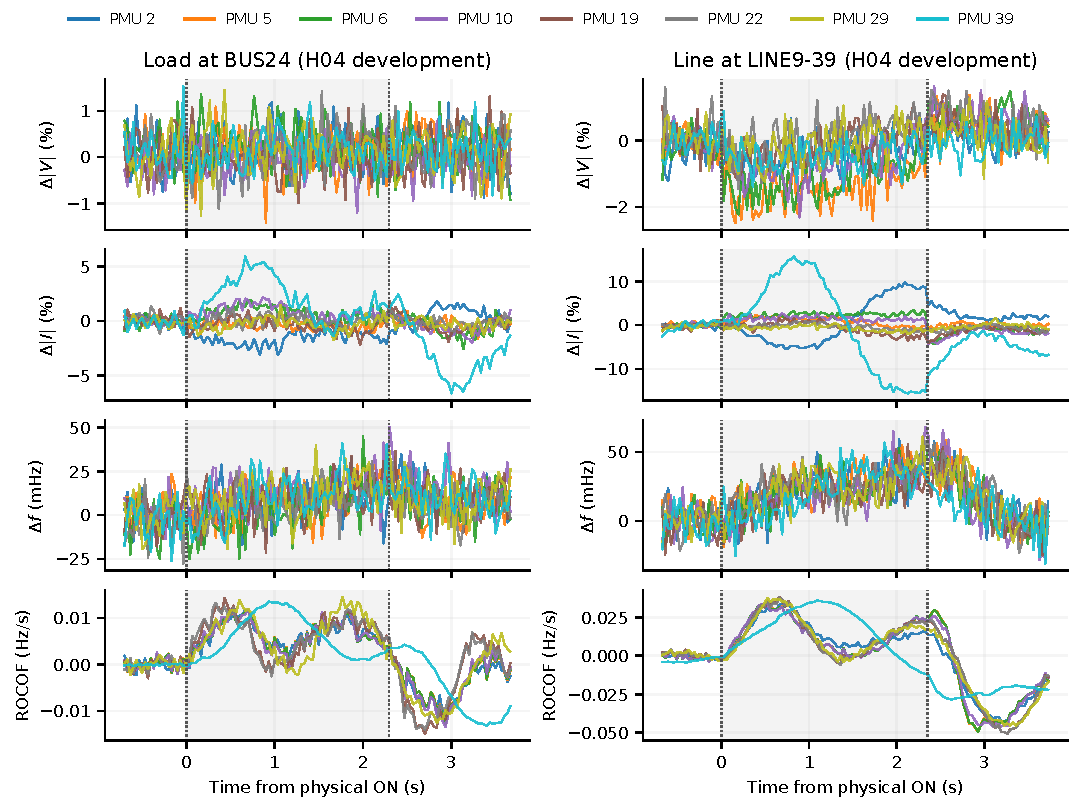
\includegraphics[width=.96\textwidth]{figures/generated/narrative_signals.pdf}
\caption{Simulated observations supplied to inference. One fixed development parent provides a load and a line example at all eight PMUs. Shading marks physical ON--OFF for evaluation only. Magnitude changes use the local pre-event center; frequency is centered for display while its exported channel remains absolute Hz. Source, severity and operating context affect the curves, so they are not universal class templates.}
\label{fig:narrative-signals}\end{figure*}

\subsection{Represent Fixed Network Uncertainty}

The bank contains nominal, global $\pm2\%$, and selected-branch $\pm3\%$
paired R/X hypotheses. Parameters stay constant within a hypothesis. Its
outer weight uses a predictive density formed before the current-report
state update and proposal selection:
\begin{equation}
 w_{\ell,k}=\frac{w_{\ell,k-1}p_\ell(y_k\mid\mathcal F_{k-1},\widehat b_\ell)}
 {\sum_jw_{j,k-1}p_j(y_k\mid\mathcal F_{k-1},\widehat b_j)}.
 \label{eq:continuous-weights}
\end{equation}
Startup-fitting reports are not scored again as independent model-selection
evidence. The mixture covers a finite set of network alternatives rather
than identifying a continuous impedance posterior.

\subsection{Keep Recovery as a Competing Physical Explanation}

Restoring an input or topology at $\kappa$ does not restore the pre-event
state: $x(\kappa^+)=x(\kappa^-)$. On a regular local post-restoration chart,
the difference from a same-context no-new-intervention trajectory obeys
\begin{align}
 \delta x_h(t)&\simeq\Phi_0(t,\kappa)\delta x_h(\kappa),\nonumber\\
 \delta y_h^{\rm net}(t)&\simeq C_0(t)\Phi_0(t,\kappa)\delta x_h(\kappa),
 \quad t>\kappa.
 \label{eq:recovery-response}
\end{align}
Here $y^{\rm net}$ denotes voltage/current coordinates before the instrument map.
Instrumental memory is retained as well. This local interpretation of known
dynamics explains why the reference after OFF is a trajectory, not a zero
residual; it is not a new propagation theorem.

For conditional history mass $\pi_{\ell,h,k}$, define active and
originating-cause masses for an admissible family/source cell $c$:
\begin{align}
 M_{c,k}&=\sum_\ell w_{\ell,k}\sum_{h:c(h)=c}
       \pi_{\ell,h,k}\,\mathbf1\{h\text{ active at }k\},\nonumber\\
 \Gamma_{c,k}&=\sum_\ell w_{\ell,k}\sum_{h:c(h)=c}\pi_{\ell,h,k}.
 \label{eq:active-cause-masses}
\end{align}
A retained history can stop being active while its cause still explains
recovery. Later interventions compete with those histories. The
implementation stores 18 admissible cells, not every family at every bus.

Writing the conditional active mass as $M_{\ell,c,k}$ yields
\begin{align}
 \Delta M_{c,k}&=\sum_\ell w_{\ell,k}
               (M_{\ell,c,k}-M_{\ell,c,k-1})\nonumber\\
 &\quad+\sum_\ell(w_{\ell,k}-w_{\ell,k-1})M_{\ell,c,k-1}.
 \label{eq:continuous-delta}
\end{align}
The terms distinguish within-model evolution from model reweighting.
This accounting identity aids interpretation, without constituting a new
tensor factorization. The masses are approximate attribution weights;
probability calibration and globally optimal filtering are not established.

\subsection{Emit Separate Detection, Diagnosis and Restoration Messages}

The fixed publication rules require active mass 0.99 for six reports to
confirm an alarm, and restoration mass 0.99 for 15 reports to confirm OFF.
The archived source/line confirmation and episode-replacement rules
determine the public diagnosis. Every message records emission time and
the last report used. A diagnosis can be correct eventually but too late
to precede physical OFF.

The nominal comparator uses the same nominal conditional model with its
own fixed publication path. Comparing nominal and mixture tests the outer
network bank. The admission-rule ablation tests a different publication
decision; it is not a pure recovery-memory ablation.

The computation follows six steps: initialize from the prefix; propagate
histories; propose/replay eligible onsets; score the new report once;
update masses; and emit messages while retaining recovery. The input grid
is 30 reports/s. Causality concerns report availability; wall-clock
real-time execution has not been established.

\FloatBarrier
\section{Experimental Design}
\label{sec:narrative-protocol}

The primary experiment asks whether the causal bank can attribute successive load/line interventions without confusing recovery with a new event. Development, independent evaluation and an auxiliary source-resolution experiment answer different questions and retain separate denominators.

\begin{table*}[t]\centering\small
\caption{Experimental populations and their purposes. Conditions and noise realizations repeat a physical parent rather than creating independent trajectories.}\label{tab:narrative-evidence}
\begin{tabularx}{\textwidth}{@{}lXXX@{}}\toprule
Population & Configuration & Main outcome & Interpretation\\\midrule
Continuous development & Three event parents, six interventions each; one normal parent; three network conditions & Timely family/source, extras and restoration & Open development evidence, not independent confirmation\\
Independent continuous evaluation & 18 event parents, six interventions each; 12 normal parents; three network conditions and two noise scales & Paired attribution, false alarms, delays and failures & Prespecified comparison of unchanged methods\\
Persistent-line evaluation & Nine lines, three parent repetitions; same network/noise strata & First stopping decision, source and censoring & Eligible comparison with published line-outage QCD\\
\IfFileExists{generated/ei_x02_macros.tex}{Signature component test & \EIDictionaryCases{} dictionary and \EITestPhysical{} test trajectories; four loads; three common noise seeds & Nominal, reference correction and mixed-signature correction & Known ON/OFF and family; separate from causal accuracy\\}{}
Recovery geometry control & 38 trajectories; four recovery histories and 12 correlated source-pair comparisons & Separation with known history and one uncertain severity direction & Supplied prior trajectory, onset, family and pair; not R11 performance\\
\bottomrule
\end{tabularx}\end{table*}

The simulator is the IEEE-39 Julia/PowerDynamics research candidate F01. Each physical parent is integrated continuously, preserving differential states through ON/OFF. Its PMU reporting grid is separate from solver steps: a 120-s record contains 3601 reports per PMU and a 600-s normal record contains 18001, including endpoints. At a switch-aligned report the export uses the post-switch algebraic value. Measurement references, load law and stochastic instrument parameters are fixed across events. RAW0001 supplied retrospective calibration context, not independent test data.

H03 and H04 each contain three event parents with six successive load/line interventions and one normal parent, all 80 s long. Schedules are paired across nominal, in-bank R/X and mixed out-of-bank R/X conditions. Each campaign therefore has 18 unique interventions and 54 event realizations. Both campaigns are now development evidence. No interval or generalization claim treats those 54 realizations as independent events.

R11 and its nominal version are frozen co-references. Both ExtraTrees artifacts and their causal preprocessing/publication adapters are frozen as well; neither is retrained on H04 or C01. They receive the same 30-fps observations. This is a comparison of those operational implementations on the stated contract, not a rerun of the hackathon leaderboard.

The published physical comparator is Chen \emph{et al.}'s persistent single-line quickest-change detector \cite{chen2016quickest}. Its reduced-network covariance is marginalized to the observed PMU subset after inversion. Parallel CUSUM statistics stop at the first threshold crossing and select a line. Our declared F01 adapter uses nonoverlapping angle increments at 15 Hz, a startup-only scale/drift estimate and the fixed nominal line catalog. Its white-injection/DC assumptions do not describe all F01 instrumental effects. We preserve both matched-law implementation checks and F01 mismatch failures; no ARL guarantee is transferred to colored noise.

The eligible common test for Chen is one persistent line opening or a normal record. Its output has no load family or restoration operator. The independent campaign, C01, therefore separates continuous load/line episodes from persistent-line first-stop decisions. Early stops, wrong sources, omissions and horizon censoring remain visible.

For continuous events, an alarm is associated temporally before predicted family/source is inspected. The first unmatched alarm after ON is eligible up to the next ON, with the inherited 30-s cap. A timely joint decision requires the correct family and asset emitted before true OFF. Unmatched alarms are extras; false restorations and open episodes are reported separately. These definitions prevent an eventual correct answer from hiding a late diagnosis.

C01 specifies 18 continuous parents, 27 persistent-line parents and 12 normal parents, with three R/X conditions and instrumental-noise scales of one and two. The 171 intended physical trajectories yield 342 observed records. Conditions represent nominal parameters, perturbations represented in the bank and mixed perturbations outside it. Solver and inference failures remain in the intended denominators. Comparisons use 10,000 paired parent-cluster resamples; repeated conditions/noise do not count as independent parents. Predictions are fixed before the evaluator opens reserved truth.

Logical decision delay is measured on report timestamps. Wall-clock cost is recorded separately with hardware, process concurrency and one-thread BLAS settings; parallel execution of independent records does not make a within-record inference method real-time. \IfFileExists{generated/c01_macros.tex}{The completed independent results follow the development examples.}{The independent evaluation is in progress. The following section reports completed development results only.}

\FloatBarrier
\section{Continuous-Stream Results}
\label{sec:narrative-results}

\subsection{Timely Attribution and Extra Alarms Measure Different Outcomes}

This section uses each frozen method's original publication policy.
The common-clock physical control in Section~\ref{sec:submission-checks}
re-publishes the same history-bank outputs under a different declared rule;
its counts are a separate endpoint. The ExtraTrees rows here are the
archived R09 references, distinct from the newly fitted S01 classifier.\AIDraftingCredit{}

\begin{table}[t]\centering\small
\caption{H04 with the original publication policies. ExtraTrees rows are archived R09 comparators. Load and line columns require the correct family and source emitted before OFF. The 54 realizations repeat 18 interventions across three R/X conditions; they are not 54 independent trials. Normal exposure is only 204 s per method.}
\label{tab:narrative-results}
\setlength{\tabcolsep}{3pt}\begin{tabular}{lrrrr}\toprule
Method & \shortstack{Load\\timely} & \shortstack{Line\\timely} & Extras & \shortstack{Normal\\alarms}\\\midrule
Physical (5 models) & 26/27 & 27/27 & 4 & 0\\
Physical nominal & 27/27 & 27/27 & 7 & 0\\
Archived ET ref. & 0/27 & 27/27 & 3 & 0\\
Archived ET short & 0/27 & 27/27 & 3 & 0\\
Onset witness & 25/27 & 27/27 & 0 & 0\\
\bottomrule\end{tabular}\end{table}


In H04, both ExtraTrees adapters and both physical references identify all tested lines in time (Table~\ref{tab:narrative-results}). The difference is in loads: the five-model bank obtains \NarMixLoadTimely{}/\NarMixLoadTotal{} timely decisions, nominal \NarNomLoadTimely{}/\NarNomLoadTotal{}, and these ExtraTrees adapters \NarETLoadTimely{}/\NarETLoadTotal{}. This tests transfer of the frozen adapters; it neither rules out supervised load detection nor reproduces the historical multi-class hackathon score.

The five-model bank detects and eventually attributes \NarMixJoint{}/\NarMixEvents{} realizations, but only \ContMixTimely{} diagnoses precede physical OFF. Nominal has \ContNomTimely{} timely diagnoses, with \ContNomExtras{} extras versus \ContMixExtras{}. Detection, eventual attribution and timely attribution therefore give different answers. The configured five-model procedure yields one fewer timely diagnosis and three fewer extra alarms than nominal; this comparison does not isolate model uncertainty.

\subsection{Recovery and a New Event Must Remain Competing Explanations}

Figure~\ref{fig:narrative-rolling} shows what the counts omit. The physical state continues evolving after OFF. Retained cause/recovery histories explain that trajectory without resetting the network; a later source must compete against both no-new-event recovery and other interventions.



The out-of-bank BUS31 case shows a remaining timing failure: the source is recovered eventually but too late. The network mixture changes how much mass is assigned to that source, and \eqref{eq:continuous-delta} separates that revision from within-model evidence. This decomposition distinguishes changing within-model evidence from changing network weights; it is an interpretation of the delayed decision.

\begin{figure}[!htbp]\centering
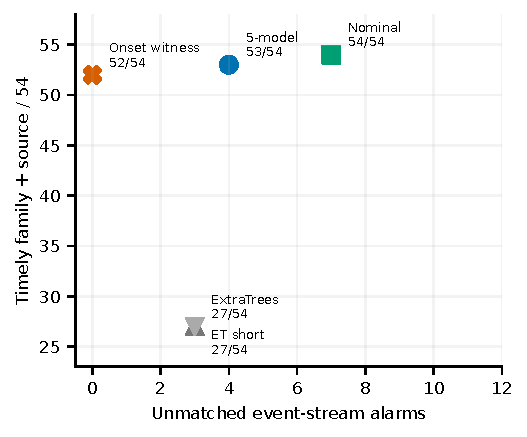
\includegraphics[width=\columnwidth]{figures/generated/narrative_tradeoff.pdf}
\caption{The decision that an accuracy-only table hides. H04 development outcomes trade timely attribution against unmatched event-stream alarms. The onset-witness ablation removes all extras but loses a real BUS16 intervention; it is retained as negative evidence. Labels use 54 paired realizations of 18 interventions and do not imply 54 independent trials.}
\label{fig:narrative-tradeoff}\end{figure}

The onset-witness ablation obtains zero extras but only \ContAdmissionTimely{}/\ContAdmissionTotal{} timely attributions: weak early evidence rejects a real BUS16 load. It inherits the physical states and masses, so suppressing the alarm does not repair the underlying explanation. This negative experiment leaves R11 and nominal frozen for C01.

\begin{figure*}[p]\centering
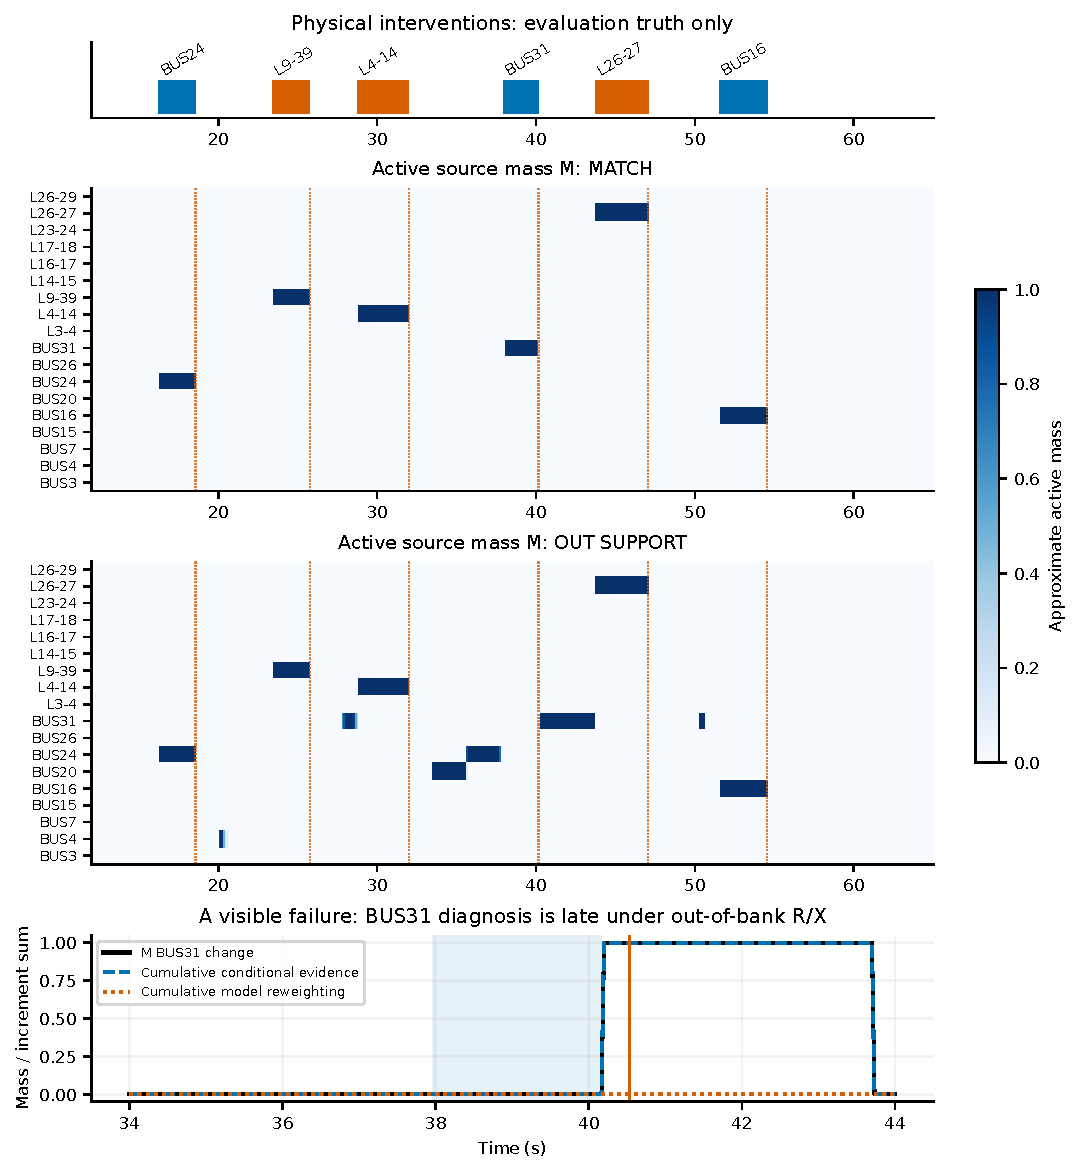
\includegraphics[width=.95\textwidth]{figures/generated/narrative_rolling.pdf}
\caption{From a continuous sequence to source attribution. Top: reserved physical ON--OFF intervals in development parent H002. Middle: active masses for nominal-network observations (MATCH) and mixed R/X changes outside the bank (OUT SUPPORT). Orange dotted lines mark true OFF for evaluation only. Bottom: BUS31 in the latter record; the cumulative terms of $\Delta M$, rebased at 34 s, sum to the change in active mass. Diagnosis arrives after OFF. The figure shows an eventual correct source that fails timely attribution; the color scale represents approximate mass, not calibrated probability.}
\label{fig:narrative-rolling}\end{figure*}

\IfFileExists{sections/08c_c01_confirmatory.tex}{\input{sections/08c_c01_confirmatory}\FloatBarrier}{}
\section{Why Visible Events Can Have Ambiguous Sources}
\label{sec:narrative-information}

The continuous results raise a separate physical question: can these
measurements distinguish the candidate sources at all? A good state
estimate does not answer it. Different interventions can produce similar
histories after fitting their severity and initial state
\cite{eriksson2013diagnosability,scharf1994matched}.

For a response $s_h$ at a specified severity and context, its distance to
an admitted competitor is
\begin{equation}
 d_h^2=\min_{j\ne h}\ \min_{\eta_j\in\mathcal A_j}
      \|s_h-s_j(\eta_j)\|_{\Sigma^{-1}}^2.
 \label{eq:narrative-separation}
\end{equation}
The set $\mathcal A_j$ specifies allowed severity, sign and nuisance
coordinates. If zero severity is admitted, different support families can
meet at the no-event boundary. Unrestricted amplitude minimization would
then give a misleading source-separation interpretation. Under a common
Gaussian law, coincident means cannot be distinguished at that
intersection. Small distances indicate a noise-sensitive problem, not a
universal error formula or an online uncertainty certificate.

A separate completed load-only experiment illustrates this limit. It uses
32 rectangular voltage/current coordinates, known onset and known operating
context. Its original amplitude-marginalized batch likelihood compares 137
zero-, one- and two-source supports on \GlobalPhysicalTrajectories{} fresh
nonlinear trajectories. It is a different estimator and evidence contract
from the causal bank.

\begin{figure*}[t]\centering
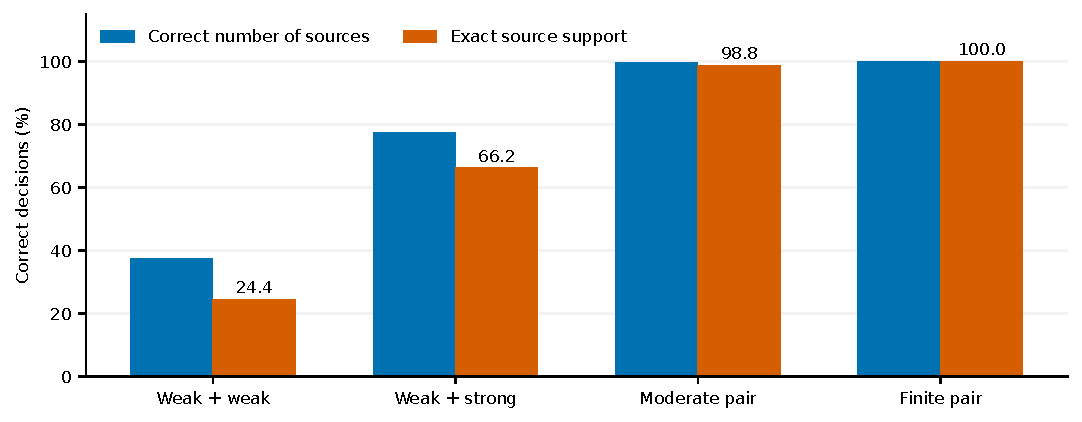
\includegraphics[width=.93\textwidth]{figures/generated/narrative_resolution.pdf}
\caption{Auxiliary source-resolution evidence, separate from the continuous estimator. In the known-onset load study, cardinality identifies the number of sources and exact support identifies their locations. Both improve with severity, but weak pairs remain difficult. These are results of the original 137-support batch likelihood, not unknown-onset R11 accuracy or a test of other event families.}
\label{fig:narrative-resolution}\end{figure*}

Exact-support Top-1 increases from \GlobalWeakTopOne{} for weak pairs to
\GlobalFiniteTopOne{} for finite pairs (Fig.~\ref{fig:narrative-resolution}).
A visible intervention therefore need not yield a reliable location.
Longer history can help separate trajectories, without guaranteeing unique
attribution for every source, severity or sensor placement. This analysis
interprets ambiguity; it is not a calibrated abstention rule in R11.
Detailed state-reconstruction studies remain supporting evidence rather
than extra event-diagnosis scores.

\FloatBarrier
\section{Interpretation and Limitations}
\label{sec:discussion}

The physical bank explains a PMU history through interventions, states and
network hypotheses. Its distinguishing operational choice is to retain a
restored intervention as a possible cause of the continuing response.
This makes recovery compete with a later event instead of treating every
departure from a flat baseline as new. The nominal/mixture comparison
shows a trade-off in development: fewer extras can accompany a late source
decision. Stricter admission eliminates extras but can also reject a real
load. These observations support reporting timely attribution and alarm
burden together.

This construction builds on established trajectory-based diagnosis,
multiple-model filtering and sequential inference. Warner's physical
trajectory scan already handles unknown onset and sparse remote PMUs;
Adaptive Matrix CuSum provides error/delay theory for its statistical
setting. We do not inherit those guarantees or claim numerical superiority
over methods not executed on common data. The present admission ablation
also does not isolate the causal benefit of every recovery-state operation.

The executed scope is a known catalog of nine loads and nine lines, with
an intervention-free startup. Missing PMUs, unknown event families,
source-excluded transfer and field operation are not tested. F01's
measurement map includes the provisional BUS5 current terminal and excludes
BUS39 current angle. Agreement with this research model does not establish
the original producer's CT placement or exact replication of RAW0001.
Local predictors, pruning, shared covariance approximations and plug-in
startup estimates limit the interpretation of the masses as probabilities.

The ExtraTrees comparison concerns two specific fixed causal adapters.
Their load-transfer failure is not evidence that supervised learning is
incapable of recognizing loads, and its score cannot be substituted for a
historical multi-family benchmark. Chen's F01 adapter has DC/white-injection
assumptions that do not capture all instrumental effects; its failures
must be reported with that mismatch.

Physics-derived stochastic priors offer a coherent direction for future
prediction uncertainty \cite{ensaf2023kernel,tartakovsky2023gp}, while
joint DAE parameter estimation addresses another task \cite{albustami2026dae}.
Such extensions would require separate validation. They are not components
silently added to the method evaluated here. The current scientific claim
rests on the specified recovery-aware mechanism and the evidence produced
by its fixed experimental contract.

\section{Conclusion}
\label{sec:conclusion}

Restoring an operator does not erase the dynamic state it created. We used
that physical distinction to construct a causal attribution bank for sparse
PMUs: load/line histories start from estimated past states, retain their
originating cause during recovery, and compete under fixed network
hypotheses. $M$ summarizes active-source mass; $\Delta M$ separates
within-model evolution from network reweighting.

\IfFileExists{generated/c01_macros.tex}{The independent continuous evaluation gives \COneMixTimely{}/\COneMixTotal{} timely family/source decisions with \COneMixExtras{} extras for the mixture, and \COneNomTimely{}/\COneNomTotal{} with \COneNomExtras{} extras for nominal. Stratified results and paired intervals determine where each choice is useful.}{Completed development streams give \ContMixTimely{}/\ContMixTotal{} timely family/source decisions with \ContMixExtras{} extras for the mixture. Nominal gains one timely decision at a higher alarm burden. Independent confirmation remains in progress.}
The auxiliary archive motivates a complementary question: how much source
ambiguity comes from the observations, approximation and evidence implementation?
Its normalization audit prevents treating an archived score as a certified
physical limit. The continuous results support a restricted study of successive load/line
attribution, rather than an all-family or universally optimal estimator.


\section*{Acknowledgment}
OpenAI Codex assisted with drafting and restructuring the main text,
LaTeX preparation, and plotting and execution-infrastructure code.
The authors retain responsibility for the scientific content, verification,
and final submission.
\FloatBarrier
\bibliographystyle{IEEEtran}
\bibliography{references}

\EOD
\end{document}
